\documentclass[10pt]{article}
\usepackage[margin=1.2in]{geometry} % change page margin
\usepackage{graphicx} % display pictures
\usepackage{amsmath}  % math modes like 'align'
\usepackage{fancyvrb} % pretty spaces in verbatim
\usepackage{hyperref}
\usepackage[linesnumbered]{algorithm2e}
\usepackage{xcolor}

\title{POSIT, final report}
\author{
  Shay Agroskin \\
  \texttt{agroskinshay@campus.technion.ac.il}
  \and
  Shahaf Haller \\
  \texttt{hallershahaf@campus.technion.ac.il}
}


\begin{document}

\maketitle

\tableofcontents

\pagebreak

\section{Abstact}\label{sec:abstact}

This project studies and implement the a floating point format called POSIT. It
explains the differences between the POSIT and the current industry standard in
terms of implementation complexity and computation accuracy.
\autoref{sec:impl-overv} describes the implementation of different arithmetic
units for the new format using SystemVerilog.

\paragraph{}
The project concludes that the new format is more suitable for
workflows that need high accuracy and don't need to represent high range of
numbers. Combined with the implementation simplicity, the new format can be a
candidate to replace the current IEEE 754 standard.

\section{Introduction}\label{sec:introduction}

The project analyzes a new way to do fractions arithmetic, instead of
the standard floating point implementation used today.

Fraction arithmetic efficiency and accuracy draws more attention in recent years
due to the growing popularity of machine learning and more complex graphic
designs (e.g.\ video games). While some approaches propose different
implementations of the current IEEE standard, other studies suggest a different
way to represent fractions all together.
This project studies one of these new formats called POSIT\cite{gustavson}.\@

\subsection{Floating points}\label{sec:floatingpoints}

The current industry standard for fraction representation is the IEEE standard
754 (floats), in which a fraction is represented by three fields: sign, exponent
and significant (see \autoref{fig:ieee754}). By denoting the sign as s, the exponent as e and significant
as f, the decimal representation of the number is represented by:


\begin{align}
  {(-1)}^{s} \cdot 2^{e - bias} \cdot 1.f\label{eq:1}
\end{align}

\noindent The range and precision of numbers that can be represented using this format
along with the value of \textit{bias} depend on the vector's length. The
standard defines 3 types of vector lengths:

\begin{table*}[h]\centering

      \begin{tabular}{|l|l|l|l|l|}
      \hline
      & vector & exponent & fraction & bias \\
      & length & bits & bits & \\
      \hline
      half & 16 & 5 & 10 & 15 \\
      precision & & & & \\
      \hline
      single & 32 & 8 & 23 & 127 \\
      precision & & & & \\
      \hline
      double & 64 & 11 & 52 & 1023 \\
      precision & & & & \\
      \hline
    \end{tabular}

\end{table*}

\noindent{}The most used lengths nowadays are a 32 and 64 bit vectors.

\begin{figure}[h]
  \centering
  \includegraphics*[width=\textwidth, height=1.5cm]{ieee_754_format}
  \caption{IEEE 754 standard fraction representation}\label{fig:ieee754}
\end{figure}

\noindent{}For example, the number 1.5 can be represented by setting $s=0, e=bias, f=1.5$ since
\begin{align*}
  (1.5)_{10} = (1.1)_{2} = (-1)^{0} \cdot 2^{bias - bias} \cdot 1.5
\end{align*}

\noindent{}As seen in \autoref{eq:1}, the \textit{significant} only specifies the
fractional part of the number ``$1.significant$''. In our example, this implies that
the value \textit{f} would be represented by $0.1$ in the floating point vector.

\subsubsection{Special values}\label{sec:special-values}

The format reserves some special values with different meaning:
\begin{itemize}
  \item Zero - zero is a special value denoted with an exponent and fraction of
  0. The format distinguishes between $+0$ and $-0$ using the \textit{sign} bit.
  Although each has its own representation, both zeroes are equal.
  \item Denormalised - If the \textit{exponent} is all zeroes, but the
  \textit{fraction} is not, then the value is a denormalized number. This means
  that this number does not have an assumed leading one before the binary point:
  \begin{align*}
    (-1)^{sign} \cdot e^{-bias} \cdot 0.fraction
  \end{align*}
  \item Infinity - The value $\pm \infty$ are denoted with an \textit{exponent} of all
  ones and a \textit{fraction} of all zeroes. The sign bit distinguishes between
  negative and positive infinity. Every multiplication and addition with the
  infinity value would result in infinity except multiplication by 0 which would
  result in NAN.
  \item Not A Number (NAN) - The value NAN is used to represent a value that is
  an error. This is represented when \textit{exponent} field is all ones with a
  zero sign bit and \textit{fraction} field that is not zero.

\end{itemize}

\autoref{tab:ieee754_special_vals} summarizes the representation of the IEEE 754
special values.

\begin{table}[h]\centering
  
  \begin{tabular}{|l|l|l|}
    \hline
    Exponent & Fraction & value \\
    \hline
    0 & 0 & 0 \\
    \hline
    all set & 0 & $\pm \infty$ \\
    \hline
    0 & not 0 & denormalized \\
    \hline
    all set & not 0 & Not A Number (NAN) \\
    \hline
  \end{tabular}
  
  \caption{Summary of IEEE 754 special values}
  \label{tab:ieee754_special_vals}
\end{table}

\subsection{Caveats}\label{sec:floatscaveats}

Although ubiquitous, the IEEE standard 754 has several downsides. Since the
exponent and fraction bit lengths are fixed, the range and accuracy of a number
that can be represented using this format are limited, which in turn case some
problems.

\subsubsection{Representation problem}\label{sec:accuracyproblem}

The IEEE standard 754 requires choosing the base of the exponent part and the
number of bits to represent it during implementation. Regardless of the chosen
base, some number would always be impossible to represent exactly.

For example, by choosing base 2, the number $0.3$ cannot be represented
precisely and is rounded to a value that can be represented by
\begin{align*}
  {2}^{e - bias}\cdot 1.f
\end{align*}

\noindent{}Since $0.3$ representation is only and approximation of the real number, the
following Python code
\begin{verbatim}
> 0.3 + 0.3 + 0.3 == 0.9
\end{verbatim}
is mistakenly evaluated to ``False''.

\subsubsection{Granularity and Range problem}\label{sec:gran-range-probl}

The range and precision of an IEEE 754 number depend on the number of bits
allocated to it during implementation.
Allocating more bits to the exponent part can the range of numbers, while
increasing the \textit{fraction} field can increase their accuracy.
For example, to represent the number $\frac{1}{3}$ we need infinite bits for the
fraction part.

Moreover, as the \textit{exponent} value increases, the precision granularity
gets worse (as seen in \autoref{prec_value}) since each change in the
\textit{fraction} part is multiplied by the \textit{exponent} value (see
\autoref{eq:1} for reference).

This creates a situation where precision-sensitive workflows need to settle on
the given \textit{fraction} bits, even when the big range is not required (since
the fraction part cannot use the exponent bits to increase precision).

\begin{figure}[h]
  \centering
  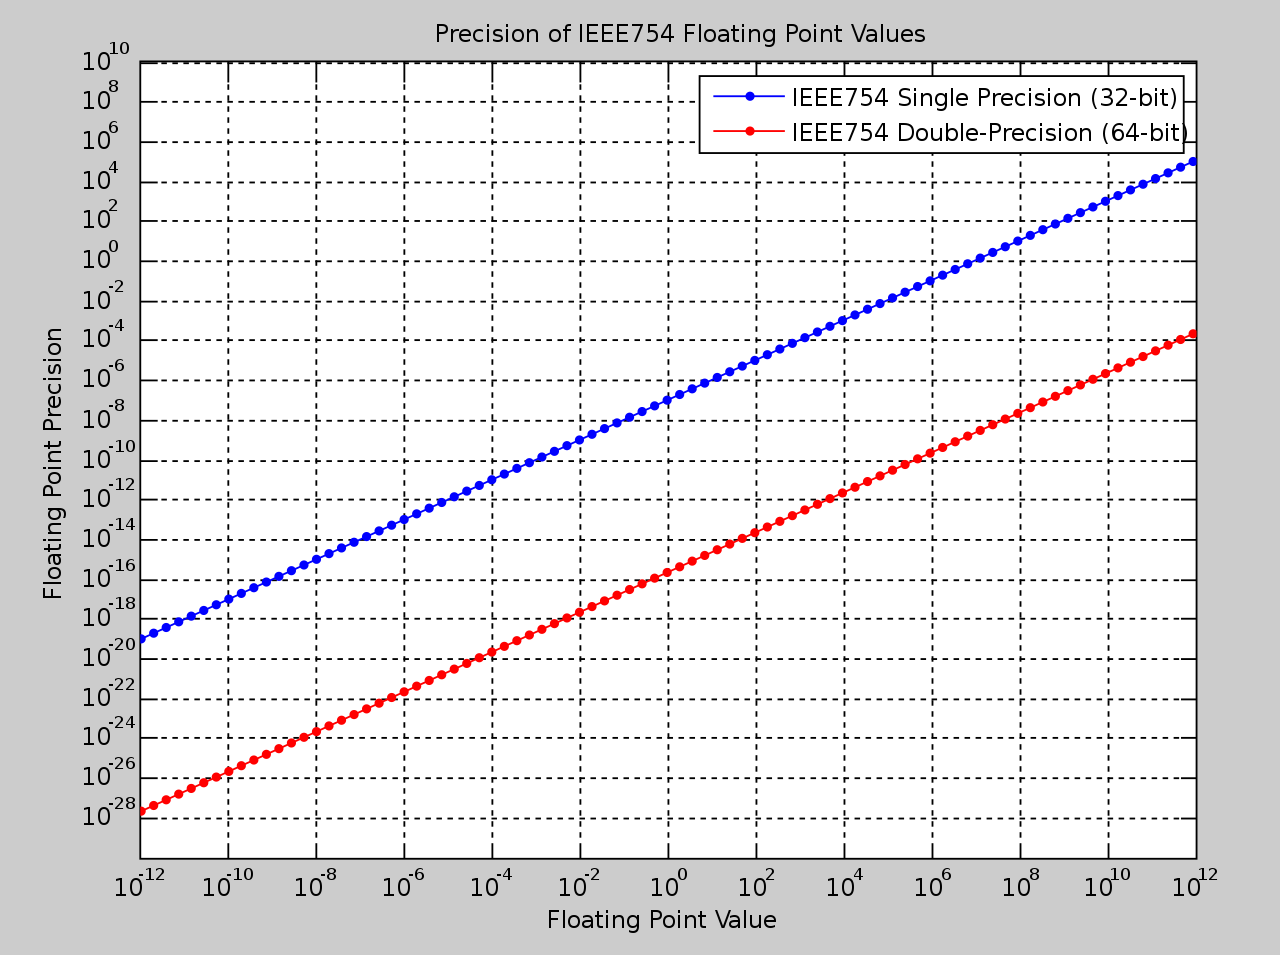
\includegraphics[width=\textwidth, height=0.3\paperheight]{1280px-IEEE754}
  \caption{Precision for different float values}\label{prec_value}
\end{figure}

\subsubsection{Wasteful representation}\label{sec:wast-repr}

There are more than one way to represent the same number using the existing
format. As explained in \autoref{sec:special-values} the NAN number are
represented by setting the \textit{exponent} bits to zero and \textit{fraction}
bits to not zero. In single precision format, this leads to
$2\cdot (2^{23} - 1)$ different representation of NANs. \\
Since all NAN are the same, this representation is quite wasteful.

\section{POSIT}\label{sec:posit}

In order to tackle some of the IEEE 754 format's problems, a new format was
proposed by John Gustavson which is called POSIT\cite{gustavson}.\@

The new format divides the bit vector into four parts (\Ref{fig:posit_format}):
\textit{sign, regime, exponent} and \textit{fraction}, which together form the
decimal number:
\begin{align}
{(-1)}^{sign} \cdot ({useed}^{regime}) \cdot {2}^{exponent} \cdot 1.fraction \label{eq:2}
\end{align}

\noindent{}where $useed = 2^{2^{es}}$ and \textit{es} is the number of bits used for the exponent part.

\begin{figure}[h]
  \centering
  \includegraphics*[width=\textwidth]{POSIT_format}
  \caption{Generic posit format for finite, nonzero values}\label{fig:posit_format}
\end{figure}

\subsection{regime value}\label{sec:regime-value}

The \textit{regime} value depends on the running sequence starting after the sign bit in the
following manner:
\begin{align*}
  bbbbbbb\overline{b}
\end{align*}

\noindent{}in this sequence of n \textit{b}'s and one \textit{$\overline{b}$}
\begin{itemize}
  \item if b=0, the regime equals to -n
  \item if b=1, the regime equals to n-1
\end{itemize}
Figure \Ref{fig:regime_values} shows more examples of \textit{regime} sequences and their
value in the \autoref{eq:2}:

\begin{figure}[h]
  \centering
  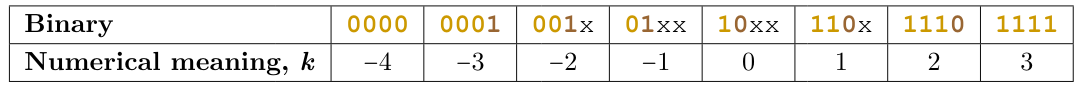
\includegraphics[width=\textwidth, height=0.04\paperheight]{regime_values}
  \caption{Different regime sequences and their respective value}\label{fig:regime_values}
\end{figure}


\subsection{Dynamic range and accuracy}\label{sec:dynam-range-accur}

As explain the \textit{regime} description in \autoref{sec:regime-value}, the \textit{regime}
field does not have a fixed size: The number of bits in the regime part are
determined by the first flipped bit after the bit sequence. \\\\
This implies that both \textit{01} and \textit{111111111111110} are valid regime sequences
(equal to $-1$ and $13$ respectively) which can be part of a 32bit POSIT vector.
In fact, the regime sequence can take up to the whole POSIT bit vector.
Since the exponent field size is fixed, the fraction bit width change according
the regime part.

If no flipped bit exists, meaning that the POSIT vector has to form of
\textit{$sbbbbbbbbb$} where \textit{s} is the sign bit, then the POSIT vector
receives a special value depending on the value of \textit{b} and \textit{s}
(see \autoref{sec:posit-speciel-values} for more information).

\paragraph{}
The dynamic field size help with the granularity and range problem
(\ref{sec:gran-range-probl}) by allowing workflows to use large regime
fields when working with very large number and small regime fields when in need
of high accuracy (the size of the fraction field is implied by the regime part).

\subsection{exponent and fraction fields}\label{sec:expon-fract-fields}

The \textit{exponent} field width, denoted as \textit{es}, is fixed and determined at
implementation. The field's starts after the first flipped bit that marks the
\textit{regime} field's end (see \autoref{sec:regime-value}). If there are less
than \textit{es} bits left after the \textit{regime} field, the
\textit{exponent} field is right-padded with zeroes.

Unlike the IEEE 754 standard, in POSIT the \textit{exponent} field represent a
positive number without \textit{bias}. This implies that the \textit{exponent}
range is $0 \leq exponent \leq 2^{es} - 1$

\subsubsection{fraction field}\label{sec:fraction-field}
The \textit{fraction} part of the POSIT starts after the \textit{exponent} field
(see \autoref{fig:posit_format}) and its width depends on the number of bits
occupied by the \textit{sign}, \textit{regime} and \textit{exponent}
parts(\Ref{sec:regime-value}).

\paragraph{}
Like the IEEE 754 format, the POSIT format assumes that the \textit{fraction} field only
describes the fractional part of a number $1\leq n < 2 $. For example, the
decimal representation of the \textit{fraction} field $b_{1},b_{2},\dots,b_{n}$
is:
\begin{align*}
 1 + \sum_{i=1}^{n}b_{i}\cdot 2^{-i}
\end{align*}

Combining the \textit{sign}, \textit{regime} and \textit{exponent} parts the
decimal representation of a POSIT vector is

\begin{align}
  \label{eq:3}
  {(-1)}^{sign} \cdot ({useed}^{regime}) \cdot {2}^{exponent} \cdot 1.fraction
\end{align}


\autoref{fig:diff_posit_vals} shows different POSIT vectors and their decimal
value. As the figure shows, in case the fraction part is absent, it is assumed
to be zero (i.e. its decimal representation is $1 + 0 = 1$)

\begin{figure}[h]
  \centering
  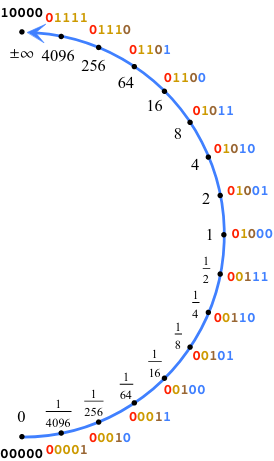
\includegraphics[height=0.25\paperheight]{posit_values}
  \caption{5-bit POSIT vectors with \textcolor{blue}{es} = 2, \textcolor{brown}{useed} = $2^{2^{es}} = 16$ and their
    decimal value}
  \label{fig:diff_posit_vals}
\end{figure}

\subsection{POSIT special values}\label{sec:posit-special-values}

Similar to IEEE 754 the POSIT format defines special values:
\begin{itemize}
  \item infinity -POSIT format does not differentiate between $\pm\infty$ and
    represents them both by setting the \textit{sign} bit and clearing the rest
    of the vector (as can be seen in \autoref{fig:diff_posit_vals}).
  \item zero - a vector with all its bits cleared represents the zero value.
    POSIT has only representation for it.
  \item regime only number - if the \textit{regime} part consists of striding 1's and has
    no flipped bit, then the vector is assumed to have \textit{exponent} and
    \textit{fraction} part equal to 0, and the \textit{regime} field is assumed
    to have flipped bit at its end. For example, for a 16 bit POSIT vector, this
    value would be represented as:
    \begin{align*}
      s111111111111111
    \end{align*}
    Where $s$ is the sign bit. In this example the number is equal to
    \begin{align*}
      (-1)^{s}\cdot (useed)^{14}
    \end{align*}
  \end{itemize}

  \autoref{tab:special_posit_value} summarizes the special POSIT values
  \begin{table}[h]\centering
    \begin{tabular}{|l|l|l|}
      \hline
      sign & the other & bits value \\
      \hline
      0 & all cleared 0 & \\
      \hline
      1 & all cleared & $\pm \infty $ \\
      \hline
      0 & all set & $(useed)^{n- 1} $ \\
      \hline
      1 & all set & $-(useed)^{n-1} $ \\
      \hline
    \end{tabular}

    \caption{Special POSIT values}
    \label{tab:special_posit_value}
  \end{table}
\paragraph{}
Unlike the IEEE 754 format, POSIT doesn't have a representation of NaN. In order
to signal that a computational result is invalid the hardware implementation of
the format should raise an interrupt.

\section{Related work}\label{sec:relatedwork}

Several models were proposed in order to do fraction arithmetic more efficiently.
This section describes some of these methods.

\subsection{Representing fractions by numerator and denominator}\label{sec:repr-fract-as}

The use of a format that specifies the \textit{exponent} part separately, e.g.
IEEE 754(\Ref{sec:floatingpoints}) or POSIT(\Ref{sec:posit}), limits
representation of numbers which that cannot be expressed using a chosen.\\ For example,
when using the IEEE 754 format with base 2, one cannot represent $\frac{1}{3}$
exactly,  since $\frac{1}{3}$ cannot be represented as a sum of $2^{-i}$ (see
\autoref{sec:posit} for more information).

\paragraph{}
One approach to represent rational numbers more accurately is to represent every
number using its nominator and denominator values. For example to represent the
number $\frac{1}{3}$ the implementation would hold the values 1 and 3.

Multiplication and division could be implemented using integer arithmetic.
Addition and subtraction would require first finding the LCM of the two
denominators before adding/subtracting the nominators.

Irrational numbers could be represented as an approximation using a rational
number e.g. $\pi \approx \frac{22}{7}$.

\paragraph{}
This method already has some software implementations, for example
\textit{Fraction} data type.

\subsubsection{Caveats}\label{sec:caveats}

Frequent fraction additions with the use of \textit{lcm} (different
denominators), might result in a too large denominator and might require the use
of the \textit{gcd} algorithm to reduce it.

This would result in a very complex implementation with high latency per each
arithmetic operation, and might not be suitable for many performance centered workflows.

\subsection{Increasing Float size}\label{sec:increasefloat}

As described in \autoref{sec:gran-range-probl}, the bits in the
\textit{fraction} field results in higher accuracy. Workflows which require high
accuracy can use a modified version of the IEEE 754 format with more bits for
the \textit{fraction} parts. This solution presents a somewhat ``quick fix'' as
it does not require to change the existing HW significantly.

\subsubsection{Caveats}\label{sec:caveats-1}

Though simple, this solution does not solve the any of the problems listed in
\autoref{sec:floatscaveats} and merely reduces the impact of some of them.
Also, increasing the total bits per float would result in increase in either
latency or power consumption.

\section{Environment and tools}\label{sec:environment-tools}

\begin{itemize}
  \item Icarus iverilog and vvp - Most of the development for this project was
  done on Linux private computers. The free \textit{iverilog} allows for a
  command line compilation of System Verilog code. The \textit{vvp} is used for
  running the compiled file.
  \item Inkscape - this tool is used to creating vector design (similar to Adobe
  illustrator, but free). It was used to designing the logic diagrams for
  various components.
  \item Synopsis tools for synthesis and elaboration - these tools were used to
  verify that the code is indeed synthesizable.
\end{itemize}

\section{Implementation overview}\label{sec:impl-overv}

Similar to Intel's ALU implementation, This project's implementation first
divides the POSIT vector into three fields \textit{regime}, \textit{exponent} and
\textit{fraction}, each of the same bit length as the original POSIT vector (as
depicted in \autoref{fig:adder_block_diagram}). For example, a 32bit POSIT
vector would be divided into three fields that are 32bit long each.

These fields represent the value of the \textit{regime}, \textit{exponent} and
\textit{fraction} parts of the vector \emph{after} they've been converted
into a 2's complement representation. \autoref{fig:adder_block_diagram}
illustrates a block diagram of the POSIT adder implementation. As can be seen
from the figure, the addition is done on each field separately and the results
are combined (``packed'') together afterwards to form a valid POSIT vector (see
``Packer'' subsubsection\Ref{sec:packer})

\begin{figure}[h]
  \centering
  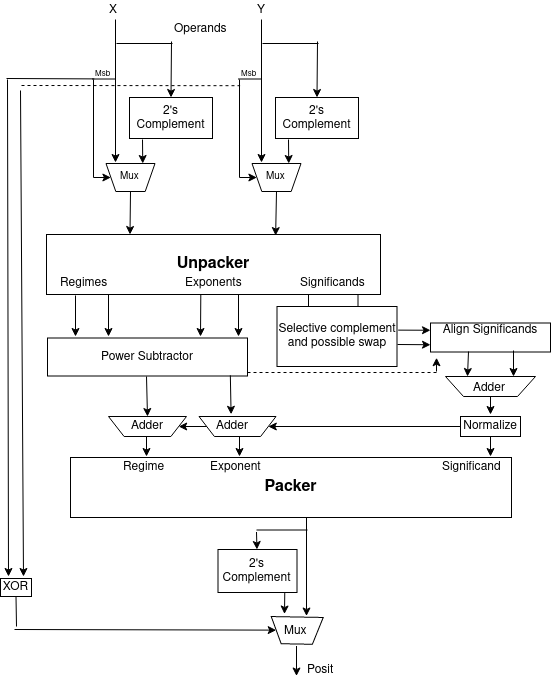
\includegraphics[width=\textwidth, height=0.4\paperheight]{adder_block_diagram}
  \caption{Block diagram of the adder module}
  \label{fig:adder_block_diagram}
\end{figure}

\subsection{Packer and unpacker modules}\label{sec:pack-unpack-modul}

As explained, in this implementation, every arithmetic operation on a POSIT
vector, is performed on each of its fields (\textit{regime}, \textit{exponent},
\textit{fraction}) separately and the results of all operations are then
combined into a new POSIT vector.

\subsubsection{Unpacker}\label{sec:unpacker}

The \textit{unpacker} module is responsible for converting a POSIT vector into
three fields that represent its \textit{regime}, \textit{exponent},
\textit{fraction} parts in 2's complement representation.

The logic gate diagram (illustrated in \autoref{fig:unpacker_diagram})
shows how the \textit{unpacker} module receives a POSIT vector of \textit{bits}
length and returns its three components.

\begin{figure}[h]
  \centering
  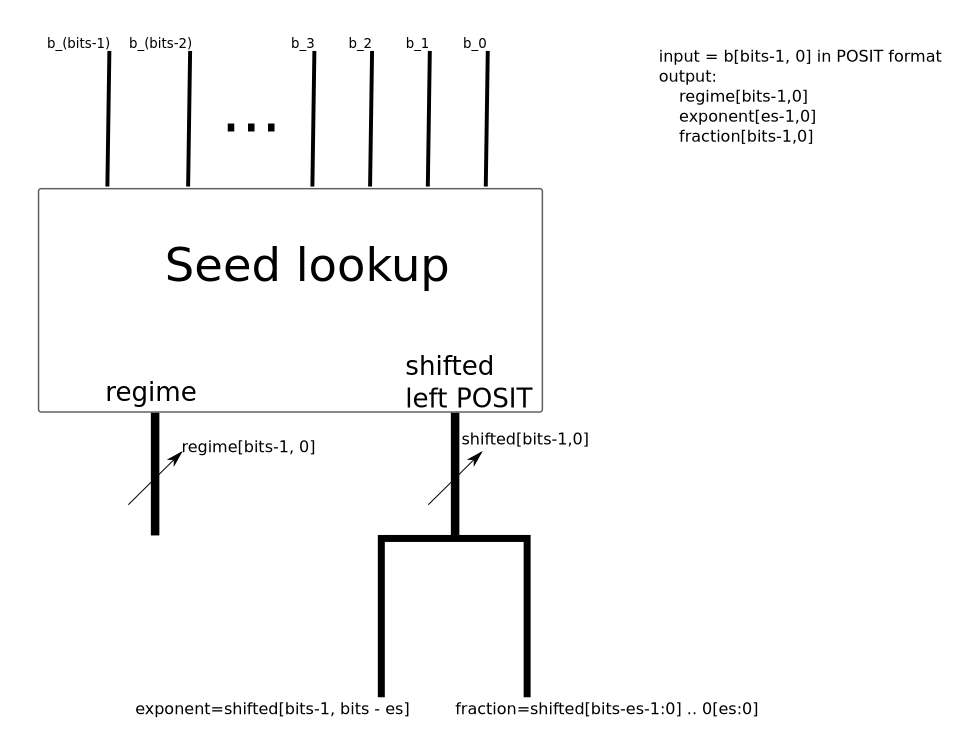
\includegraphics[width=\textwidth, height=0.2\paperheight]{unpacker_diagram}
  \caption{Unpacker diagram}
  \label{fig:unpacker_diagram}
\end{figure}

To better understand the implementation of the \textit{unpacker} module,
\autoref{fig:seed_lookup_diagram} illustrates the \textit{seed\_lookup} module
which takes a POSIT vector and by XORing all bits finds the first flipped bit
of the \textit{regime}.
Afterwards, the module uses the  \textit{regime} value to shift the POSIT vector left
so the \textit{exponent} part starts in the MSB. It does so to make it easier
for the \textit{unpacker} module to extract the other fields of the input vector.

\begin{figure}[h]
  \centering
  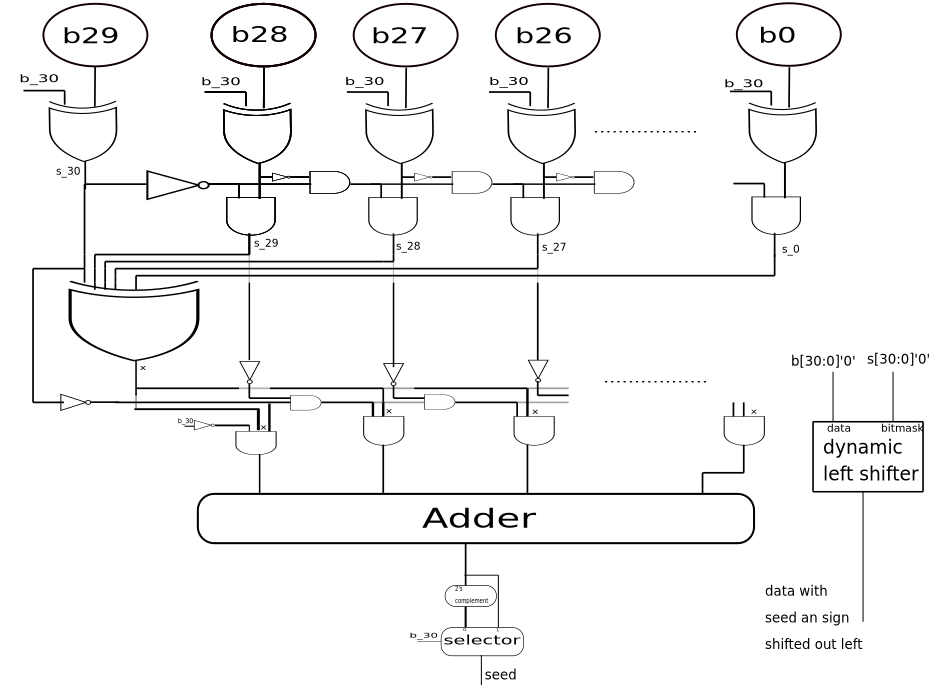
\includegraphics[width=.8\textwidth,height=0.3\paperheight]{seed_lookup}
  \caption{seed\_lookup logic gate diagram}
  \label{fig:seed_lookup_diagram}
\end{figure}

The implementation avoids using any register dependant logic to achieve low
latency.

\subsubsection{Packer}\label{sec:packer}

The \textit{packer} does the exact opposite of \textit{unpacker} module. It
receives \textit{regime}, \textit{exponent}, \textit{fraction} from the
\textit{multiplier} or \textit{adder} and creates a POSIT vector from it.
The \textit{packer} also receives an additional \textit{zero} flag which tells
it if the result of the previous module is zero.

The following pseudocode describes the verilog implementation of this module:\\

\begin{algorithm}[H]
 \KwData{seed, exponent, fraction and zero}
 \KwResult{a POSIT vector }
 \eIf{zero is set}{
   return POSIT = zero vector
 } {
   set seed\_seq = sequence of running 1s or 0s depending on sign(seed) \\
   set POSIT = seed\_seq concatenated with exponent and fraction parts \\
   return the first \textit{n} bits of the POSIT vector, where \textit{n} is the
   desired POSIT length
 }
\end{algorithm}

The extra \textit{zero} input is needed because the numbers one and zero both
have all three parts equal to 0 (i.e. $seed=0,\ exponent=0,\ fraction=0$).
This issue is discussed in \autoref{sec:pack-repr-1}.

\subsection{Multiplication and Addition}\label{sec:mult-addit}

The \textit{multiplier} and \textit{adder} modules receive two POSIT vector and return
their product and sum accordingly (as shown in \autoref{fig:adder_black_box} for
the adder).
Each of them uses the \textit{unpacker} and \textit{packer}
modules internally to decompose each of the received vectors into their
respective \textit{regime}, \textit{exponent} and \textit{fraction} fields.
The addition/multiplication is done on each of the fields separately and the
three results are combined into a single POSIT vector.

\begin{figure}[h]
  \centering
  \includegraphics*[width=0.5\textwidth, height=0.2\paperheight]{adder_blackbox}
  \caption{Adder blackbox scheme}
  \label{fig:adder_black_box}
\end{figure}

\subsubsection{Adder}\label{sec:adder}

As explained in \autoref{sec:mult-addit}, the addition starts by decomposing the
input POSIT vectors into their three components.

The \textit{adder} module can be expressed by the following pseudo-code: \\

\begin{algorithm}[H]
 \KwData{Two POSIT vectors $p_{1}, p_{2}$}
 \KwResult{vectors sum in POSIT format $p_{r}$}
 denote seed, exponent and fraction fields of the two vectors as
 $s_{1}, e_{1}, f_{1}, s_{2}, e_{2}, f_{2}$ \\
 Also denote the fields of the $p_{r}$ as $s_{r}, e_{r}, f_{r}$. \\

 \eIf{$p_{1} = \pm\infty$ or $p_{2} = \pm \infty$}{
   return $p_{r} = \pm \infty$
 } {
   $sum_{i}= s_{i} << ES + e_{i} \quad i=1,2$ \\
   \eIf{$sum_{1} > sum_{2}$ or ($sum_{1} = sum_{2}$ and $f_{1} > f_{2})$}{
     bigFrac = $f_{1}$;
     bigExpSum = $sum_{1}$ \\
     smallFrac = $f_{2}$;   
     smallExpSum = $sum_{2}$
   }{
     bigFrac = $f_{2}$;
     bigExpSum = $sum_{2}$ \\
     smallFrac = $f_{1}$;
     smallExpSum = $sum_{1}$
   }
   $resultExp = bigExpSum$ \\
   $sumDiff = bigExpSum - smallExpSum$ \\
   $resultFrac = bigFrac + (smallFrac >> sumDiff)$ \\
   \eIf{$resultFrac$ overflows}{
     resultExp = resultExp + 1 \\
     resultFrac = resultFrac / 2
   }{
     resultExp -= number of time to shift $resultFrac$ left until its $MSB = 1$
   }

   $s_{r}$ = resultExp $<<$ \textit{es} \\
   $e_{r}$ = first \textit{es} bits of resultExp \\
   $f_{r}$ = resultFrac
    }
  \end{algorithm}

  \vspace{0.3cm}
\noindent To put the algorithm in words:
\begin{enumerate}

  \item if either of the POSITs represent $\pm \infty$ (same representation, see
  \autoref{sec:posit-special-values}), set the result to be $\pm \infty$ (lines 3-4)
  \item the \textit{adder} normalizes the received vectors so that they both
    have the same exponent (seed + exponent field). The equation in line 6  equals to
    $ s_{i} \cdot 2^{es} + e_{i}$ (which is equal to
    the total exponent of the POSIT). (lines 6-16)

  \item add the normalized fraction parts and adjust the common exponent to
  reflect an overflow in the result. (lines 18-19)
  \item adjust the common exponent so that the fraction sum would be between 1
    and 2. This is needed because the fraction part in POSIT is assumed to be in
    that range. Therefore the exponent needs to be adjusted to scale the
    fraction part as needed. (line 21)
  
  \end{enumerate}

  % TODO: add some words regarding

\subsubsection{Multiplier}\label{sec:multiplier}

As oppose to the \textit{adder} module, multiplication doesn't require
normalizing the exponents before operation. The following pseudo-code describe
its operation: \\
\begin{algorithm}[H]
 \KwData{Two POSIT vectors $p_{1}, p_{2}$}
 \KwResult{vectors product in POSIT format $p_{r}$}
 denote seed, exponent and fraction fields of the two vectors as
 $s_{1}, e_{1}, f_{1}, s_{2}, e_{2}, f_{2}$ \\
 Also denote the fields of the $p_{r}$ as $s_{r}, e_{r}, f_{r}$. \\

 \eIf{$p_{1} = \pm\infty$ or $p_{2} = \pm \infty$}{
   return $p_{r} = \pm \infty$
 } {

   $s_{r}$ = $s_{1} + s_{2}$ \\
   $e_{r}$ = $e_{1} + e_{2}$ \\
   $f_{r}$ = $f_{1} * f_{2}$ \\
   \If{$f_{r}$ overflows}{$e_{r} = e_{r} + 1$}
   \If{$e_{r}$ overflows}{$s_{r} = s_{r} + 1$}
    }
  \end{algorithm}

\noindent note that is the \textit{seed} value overflows (meaning that the
POSIT vector is a \textit{sign} bit followed by a sequence of the bit), then the
output POSIT would be rounded to $\pm \infty$ or zero, depending on the sign of
the seed.

\subsection{Division and subtraction}\label{sec:division-subtraction}

Subtraction can be implemented using the same logic as addition. Similarly,
division can be regarded as a multiplication with the reciprocal of the dividing
number:
\begin{align*}
  A/B = A\cdot \frac{1}{B}
\end{align*}

\noindent The POSIT format allows an easy transformation between a POSIT and its
reciprocal value (as seen in \autoref{fig:diff_posit_vals}). The reciprocal is
obtained by 2's complementing all exponent bits (\textit{regime} +
\textit{exponent} field). To reciprocate the \textit{fraction} a different logic
should be implemented, such as translation tables (POSIT doesn't offer a fast
method to reciprocate this field).
As with IEEE 754 format, the reciprocal is only accurate up to the closest
exponent of 2.

\section{Issues encountered during the project}\label{sec:issu-enco-during}

\subsection{Packer representation of 1}
\label{sec:pack-repr-1}

Found out that by removing the leading 1 in the fraction part the
\textit{packer} module cannot tell zero and one apart.

\subsection{Non-synthesizable code}
\label{sec:non-synth-code}

After sending our code for review we realized that our verilog code is not synthesizable


\begin{thebibliography}{99}
  \bibitem{gustavson}
  Gustavson, Yonemato
  \textit{Beating Floating Point at its Own Game: Posit Arithmetic}
  \url{http://www.johngustafson.net/pdfs/BeatingFloatingPoint.pdf}

\end{thebibliography}

\end{document}

% LocalWords:  NaN
